\section{Modello entità relazioni (ER)}
Un modello dei dati è una collezione di concetti usati per descrivere i dati, le associazioni e i vincoli da rispettare.
\begin{itemize}
	\item Modello logico è usato nei DBMS per organizzare i dati e nei programmi indipendentemente dalla struttura fisica.
	\item Modello concettuale è usato per rappresentare i dati indipendentemente dall'implementazione.
	Vanta di flessibilità, intuitività e espressività.
\end{itemize}
Il modello E/R è un modello concettuale.
\subsection{Vincoli}
\begin{itemize}
	\item Ogni istanza di un'associazione deve riferirsi a istanze di entità.
	\item Istanze diverse della stessa associazione devono riferirsi a differenti combinazioni di istanze delle entità partecipanti all'associazione.
\end{itemize}
\subsection{Entità}
Classe d'oggetti della realtà di interesse che possiedono caratteristiche comuni e che hanno esistenza autonoma.

Graficamente è un rettangolo con denominazione "parlante", in maiuscolo, al singolare, univoco nello schema.

\subsection{Associazione}
Legame logico tra entità le cui istanze (ennupe) sono combinazioni delle istanze delle entità che prendono parte all'associazione.

Insieme istanze associazione è sottoinsieme del prodotto cartesiano degli insiemi delle istanze delle entità che partecipano all'associazione. \textbf{Non possono esserci istaze ripetute in un'associazione.}

Graficamente è un rombo con sostantivo e non verbi/nomi composti come denominazione (stile come le entità) .

\paragraph{Grado} della associazione è il numero d'istanze delle entità, non necessariamente distinte, che partecipano in un'istanza dell'associazione.
\subsubsection{Tipi d'associazione}
\paragraph{"Specializzata"}Tra due stesse entità si possono stabilire più associazioni con diverso significato.

\paragraph{Anello} lega un entità con se stessa (relaziona istanze della stessa identità).
Possono essere ricorsive.

Può essere simmetrica ($(a,b)\in A\to (b, a)\in A$), riflessiva ($(a,a)\in A$) e transitiva ($(a, b) \in A, (b, c)\in A\to (a,c)\in A$).
Nelle anello asimmetriche si \textbf{specifica sui rami il ruolo}, osi si esprimono i vincoli di cardinalità.
Un anello può partecipare a associazioni n-arie.

\subparagraph{Anello non ricorsiva} one-to-one o many-to-many bidirezionale/non bidirezionale.
\subparagraph{Anello ricorsivo gerarchico} one-to-many definisce una dipendenza asimmetrica che da un grafo orientato aciclico a parentalità singola.
\subparagraph{Anello ricorsivo part of} many-to-many che da un grafo orientato aciclico a paternità multipla.
\begin{paracol}{2}
	\paragraph{XOR} rende esclusiva un associazione tra un'insieme di possibili associazioni, per un istanza dell'entità.
	\switchcolumn
	\paragraph{AND} rende obbligatoria l'associazione con tutte associazioni di un'insieme, per ogni istanza dell'entità.
\end{paracol}

\medskip
Graficamente entrambe sono dei semi cerchi con nome dell'operatore che toccano gli archi tra l'entità in questione e le associazioni interessate.
\paragraph{Aggregazione} è un astrazione del concetto di parte di qualcosa e si rappresenta con un associazione (1,1) a (0, N).
\subsubsection{Cardinalità}
Associata a ogni entità che partecipa a un'associazione. Specifica (min-card, max-card) di istanze dell'associazione a cui un'istanza dell'entità può/deve partecipare.

Graficamente si indica sopra l'arco tra l'entità d'interesse e l'associazione.
Combinazioni di associazioni binarie (e1 e e2), la cardinalità minima può essere qualsiasi:
\begin{paracol}{3}
	\paragraph{uno a uno} max-card=1 per entrambe le entità.
	\switchcolumn
	\paragraph{uno a N} e1 max-card=1 e e2 max-card=N, o viceversa.
	\switchcolumn
	\paragraph{N a M} e1 max-card=1 e e2 max-card=M.
\end{paracol}
\paragraph{Terminologia} opzionale se min-card=0, obbligatoria se min-card=1, valore singolo se max-card=1, valore multiplo se max-card$>$1.
\paragraph{AIUTO} per stabilire la cardinalità minima si può pensare alla dinamica temporale della creazione delle istanze.

\subsection{Attributi}
Proprietà \textbf{elementare/semplice} di un'entità/associazione. Ha un dominio di valori.

Graficamente è un pallino bianco con denominazione, "parlante" è univoca dentro l'entità/associazione, collegato da una stangetta all'elemento di riferimento.

Gli attributi d'associazione non appartengono alle entità ma le riguardano "fortemente". CRITERIO DI SCELTA: Se un attributo dovrebbe appartenere a entrambe le entità di un'associazione allora si può dare tale attributo all'associazione.

\paragraph{Cardinalità} implicità/non scritta è (1, 1) ma può essere esplicitata con (min-card, max-card) sulla linea di congiunzione.  Un'attributo per la stessa istanza deve assumere valori distinti.

Cardinalità speciali sono: opzionale (min-card=0), monovalore (max-card=1), multivalore (max-card=N).
\paragraph{Composti} Aggregazioni di attributi elementari con forte affinità nell'uso/significato. Ha un nome "riassuntivo" dei sotto attributi.

Il dominio di un composto è il prodotto cartesiano dei domini dei sotto attributi.

I sotto attributi possono avere cardinalità specifiche indipendentemente dalla cardinalità dell'attributo composto.

Un identificatore può essere semplice (composto da un solo attributo) o composto (composto da più attributi).
\subsection{Identificato}
Individua univocamente, tramite gli attributi, delle istanze di un'entità. Un identificatore è univoco. Ogni entità deve avere almeno un vincolo di identificazione (identificatore).
\begin{itemize}
	\item semplice semplice, usa un'attributo dell'entità.

	Graficamente è un attributo con il pallino nero.
	\item Interno composto, usato più attributi dell'entità.

	Graficamente è un attributo con pallino nero che interseca gli attributi di cui si compone (tipo una chiave).
	\item Esterno/misto, usa uno o più attributi interni e esterni (delle entità associate).

	Graficamente come l'interno composto ma interseca dei segmenti che congiungono l'entità e l'arco tra l'associazione e l'altra entità.

	In questo caso è essenziale che l'entità d'interesse abbia \textbf{cardinalità (1, 1)}.

\end{itemize}
Con più identificatori gli attributi possono essere opzionali, tranne in un identificatore.
\begin{itemize}
	\item Entità deboli, hanno solo identiticatori esterni (usa anche attributi altre entità). Sia l'entità d'interesse (debole) che quella d'identificazione (dominante) devono avere \textbf{cardinalità (1, 1)}.

	Le istanze deboli accettate/esistono solo se sono presenti le istanze da cui dipendono.
	\item Entità forti, hanno solo identificatori interni.
\end{itemize}
\paragraph{Proprietà di minimalità}: Per ogni estensione ammissibile di un'entità nessun sottoinsieme proprio dell'identificatore deve essere a sua volta un identificatore.
\paragraph{Chiave primaria} uno degli identificatori dell'entità se non l'unico.

\subsection{Reificazione}
La reificazione trasforma un'associazione, con attributo composto ripetuto e identificatori, in un'entità con identificazioni esterne e associazioni binarie.

Permette di rispettare tutti i vincoli (dipendenza funzionale: $att.key\to att.$) e si sceglierà una delle chiavi primarie uno degli identificatori.
\begin{figure}[H]
	\centering
	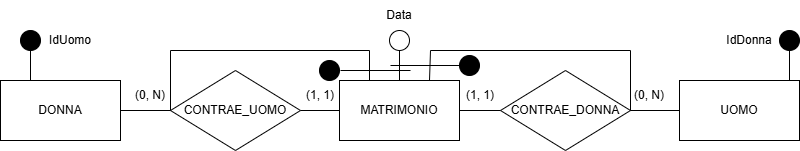
\includegraphics[width=0.9\textwidth]{img/matrimonio.png}
	\caption{Esempio di retificazione}
\end{figure}

\paragraph{La Storicizzazione} dei dati si risolve con entità legate al concetto di tempo che sono specializzazioni di altre entità. Cosi si dividono attributi statici e dinamici in entità diverse. La reificazione aiuta la storicizzazione.

\paragraph{Un associazione ternaria} o maggiore se ha dipendenze funzionali tra le sue entità deve essere reificata.
\subparagraph{Falsa ternaria} è un'associazione ternaria di cui una o più entità vi partecipa con card-max=1. Può essere rimodellata con due o più associazioni binarie con la stesssa cardinalità della ternaria.
\subsection{Generalizzazione}
Le proprietà e le associazioni del Padre sono ereditate dai Figli (non vale l'inverso). I Figli possiedono attributi e associazioni proprie.

Più generalizzazioni posso nascere dallo stesso padre. Un figlio può essere padre di una generalizzazione (gerarchia).

\textbf{Attenzione}: Le gerarchie non modellano aspetti dinamici, temporali e specifiche istante dell'entità padre.

\paragraph{La Copertura } Bisogna esplicitarla, se totale/parziale e esclusiva/sovrapposta, della generalizzazione:
\textbf{(T, E), (T, S), (P, E), (P, S)}.

\paragraph{Graficamente} si fanno congiungere dei rami dalle entità figlie in una freccia "cicciotta" affiancata dalla copertura, e che punta all'entità padre.

\paragraph{L'Ereditarietà singola} impone che in una gerarchia di generalizzazioni un Figlio abbia un solo Padre. Ciò comporta a Figli "misti" e alla replicazione degli attributi".

\paragraph{Subset} è una gerarchia con un solo Figlio per generalizzazione (is a).